\section{El paquete de Python y los bloques que lo conforman}
Python es un lenguaje de código abierto, con una comunidad activa de colaboradores y usuarios que comparten su software para que otros desarrolladores lo utilicen. Son colaboradores aquellos que comparten sus códigos o scripts, en forma de paquetes en el Python Packaging Index (PyPI). Los paquetes son similares a directorios de un sistema de archivos ya que estos permiten separar el código de forma jerárquica \cite{Paquetes}. De acuerdo con la documentación oficial, existen 3 tipos de paquetes:
\begin{itemize}
    \item \textbf{Paquetes regulares:} Son implementados como un directorio o carpeta, que contiene un archivo \mintinline{Python}{init__.py}. Cuando se importa un paquete regular, este archivo \mintinline{Python}{init__.py} se ejecuta implícitamente y los objetos que define, están vinculados a nombres en el espacio de nombres del paquete. Por ejemplo, la siguiente disposición del sistema de archivos define un paquete "parent" de nivel superior con tres sub-paquetes:
\begin{figure}[H]
    \centering
    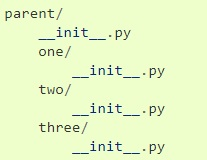
\includegraphics[scale = 0.8]{Recursos/paqueteRegular.jpg}
    \caption{Organización de directorios de un paquete regular}
    \label{PaqueteRegular}
\end{figure}
Cuando se requiere emplear un paquete es necesario primero importarlo; por lo que al importar parent.one (Ver Figura \ref{PaqueteRegular}) se ejecutará implícitamente \mintinline{Python}{parent/__init__.py} y \mintinline{Python}{parent/one/__init__.py}. 
\item \textbf{Paquetes de espacio de nombre (namespace package):} Pertenecen a esta categoría aquellos paquetes compuestos por un conjunto de archivos en un único directorio, donde cada grupo de archivos contribuye con un sub-paquete del paquete padre. A diferencia de los paquetes regulares, los conjuntos pueden estar en diferentes lugares del sistema de archivos, pueden estar en archivos .zip, en la red o cualquier otro lugar que Python busque durante la importación.
\\
Un ejemplo en donde se separa el paquete en dos distribuciones utilizando namespaces sería:
\begin{figure}[H]
    \centering
    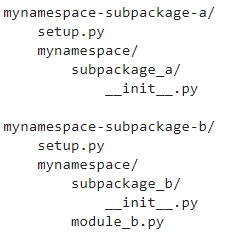
\includegraphics{Recursos/namespacePaquete.jpg}
    \caption{Organización de directorios de un paquete de espacios de nombre}
    \label{namespacePaquete}
\end{figure}
La forma de organizar el paquete utilizada en la Figura \ref{namespacePaquete} no es la única, existen otras formas donde el fichero setup.py, se encuentra en la raíz del paquete, como es el caso de los paquetes con namespace implícito \cite{PEP420}.  El fichero setup.py es aquel que permite la construcción, distribución e instalación de módulos.
\item \textbf{Paquete de importaciones relativas:} Basados en puntos iniciales. Un punto inicial indica una importación relativa, empezando por el paquete actual. Dos o más puntos iniciales indican una importación relativa a los elementos primarios del paquete actual, un nivel por punto después del primero. Por ejemplo, dado el siguiente diseño de paquete:
\begin{figure}[H]
    \centering
    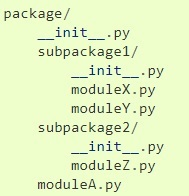
\includegraphics{Recursos/paqueteImportacionRelativa.jpg}
    \caption{Organización de directorios de un paquete de importaciones relativas}
    \label{paqueteIR}
\end{figure}
En \mintinline{Python}{subpackage1/moduleX.py} o \mintinline{Python}{subpackage1/__init__.py}, las siguientes son importaciones relativas válidas:
\begin{figure}[H]
    \centering
    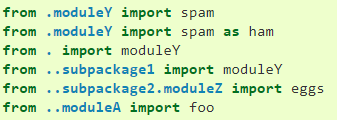
\includegraphics{Recursos/importarRelativamente.png}
    \caption{Ejemplo de importaciones relativas}
    \label{importarIR}
\end{figure}
\end{itemize}
\subsection{Módulos}
Se conoce como modulo a todo fichero o script de Python cuya extensión es .py. Separar el código en módulos permite facilitar el mantenimiento del programa a medida que crezca. Algunos aspectos a tomar en cuenta sobre los módulos serían:
\begin{itemize}
    \item Pueden contener tanto declaraciones ejecutables como definiciones de funciones. Estas declaraciones están pensadas para inicializar el módulo. Se ejecutan únicamente la primera vez que el módulo se encuentra en una declaración import\cite{ModuloPython}.
    \item Cada módulo tiene su propio espacio de nombres, el cual es usado como espacio de nombres global para todas las funciones definidas en su interior.
    \item Para optimizar la importación de módulos el autor del modulo deberá proveer un índice explícito del paquete. Esto se logra cuando el código en el archivo \mintinline{Python}{__init__.py} de un paquete define una lista llamada \mintinline{Python}{__all__.py}, dicha lista debe poseer los nombres de módulos que deberían ser importados cuando se hace \mintinline{Python}{from package import *}\cite{ModuloPython}.
\end{itemize}
\subsection{Tipos de  scripts de configuración del paquete}
\subsubsection{Distutils}
Es un paquete de Python que da soporte, para la creación, distribución e instalación de módulos, los módulos pueden ser hechos únicamente en Python o escritos en C. Distutils como paquete presenta las siguientes funcionalidades:
\begin{itemize}
    \item Soporte para declarar dependencias del proyecto, siendo las dependencias aquellos paquetes o módulos externos necesarios para el funcionamiento del proyecto.
    \item Mecanismos adicionales para configurar cuáles archivos incluir en lanzamientos de código fuente, esto se logra mediante el uso de sistemas de control de versiones.
    \item La capacidad de generar, automáticamente, ejecutables de línea de comandos de Windows en el momento de la instalación, en lugar de tener que compilarlos previamente.
    \item Comportamiento consistente en todas las versiones de Python soportadas por el paquete.
\end{itemize}
Un ejemplo de como estructurar el archivo setup.py que maneja Distutils sería:
\begin{figure}[H]
    \centering
    \begin{minted}{Python}
		from distutils.core import setup
		setup(name='Distutils',
                version='1.0',
                description='Python Distribution Utilities',
                author='Greg Ward',
                author_email='gward@python.net',
                url='https://www.python.org/sigs/distutils-sig/',
                packages=['distutils', 'distutils.command'],)
	\end{minted}
    \caption{Ejemplo de archivo setup.py utilizando el paquete Distutils}
    \label{ejDistutils}
\end{figure}
En la Figura \ref{ejDistutils} es importante resaltar la opción ``packages'' debido a que esta le dice a Distutils que procese (compile, distribuya, instale, etc.) todos los módulos de Python que se encuentran en cada paquete mencionado en la lista de "packages".
\subsubsection{Setuptools}
Es un paquete que contiene una serie de mejoras a las capacidades de Distutils, cuya cualidad principal es permitir que los desarrolladores puedan distribuir paquetes de forma más sencilla, con especial énfasis en paquetes que posean dependencias externas. Esto no implica que distutils sea obsoleto, puesto que setuptools aun se encuentra en desarrollo. A diferencia de su contra parte, las configuraciones requieren de al menos 2 archivos y un paquete, el archivo pyproject.toml; es aquel donde se debe declarar que se empleara Setuptools, este archivo debe poseer la siguiente estructura:
\begin{figure}[H]
    \centering
    \begin{minted}{Python}
		[build-system]
        requires = ["setuptools", "wheel"]
        build-backend = "setuptools.build_meta"
	\end{minted}
    \caption{Ejemplo de archivo pyproject.toml}
    \label{pyproject.toml}
\end{figure}
El archivo setup.cfg es el reemplazo al archivo setup.py y puede conformarse de la siguiente manera:
\begin{figure}[H]
    \centering
    \begin{minted}{Python}
		[metadata]
        name = "mypackage"
        version = 0.0.1

        [options]
        packages = "mypackage"
        install_requires =
        requests
        importlib; python_version == "2.6"
        
        [options.entry_points]
        console_scripts =
        main = mypkg:some_func
	\end{minted}
    \caption{Ejemplo de archivo setup.cfg}
    \label{setup.cfg}
\end{figure}
Como se puede ver en la Figura \ref{setup.cfg} el archivo es bastante similar en estructura al fichero setup.py; no obstante, tiene varias ventajas, ya que los elementos que pertenecen a la opción \mintinline{Python}{install_requires}, son directamente las dependencias del paquete, e incluso al momento de instalar un paquete externo, setuptools actualiza las dependencias necesarias. Para proyectos muy grandes es posible automatizar la busqueda de paquetes, con el fin de que no sea necesario declarar cada paquete en el fichero setup.cfg. 
Las herramientas de configuración admiten la creación automática de scripts tras la instalación mediante "\mintinline{Python}{options.entry_points}". Un paquete que emplee setuptools debe poseer la siguiente estructura de directorios:
\begin{figure}[H]
    \centering
    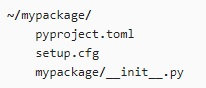
\includegraphics{Recursos/estructuraSetupTools.jpg}
    \caption{Estructura de paquete mediante setuptools}
    \label{estructuraSetupTools}
\end{figure}
El último elemento que requiere Setuptools es el paquete pep517, el cual se puede instalar mediante el instalador de paquetes de python "pip", posteriormente se debe invocar con el comando \mintinline{Python}{python -m pep517.build}.
\subsection{El paquete wheel}
Es un proyecto compatible con distutils y setuptools, que produce un formato de empaquetado binario multiplataforma (llamado ``wheels'' o ``wheel files'' y definido en PEP 427) es decir; la función de wheels es permitir la distribución de paquetes sin importar el sistema operativo empleado \cite{wheel}.
\subsection{Pruebas de regresión mediante modulo unittest}
El objetivo de las pruebas de regresión implementadas mediante el modulo unittest, es probar situaciones donde el codigo deje de funcionar, para encontrar errores en el mismo y solventar problemas en el software, de acuerdo con la documentación oficial existen una serie de pautas a seguir para ejecutar dichas pruebas, las más importantes en el caso del software a desarrollar son:
\begin{itemize}
    \item El conjunto de pruebas se debe hacer a todas las clases, funciones y constantes.
    \item Importar la menor cantidad de módulos posible. Esto minimiza las dependencias externas de las pruebas y también minimiza el posible comportamiento anómalo de los efectos secundarios de importar un módulo.
    \item Maximizar la reutilización del código. En ocasiones, las pruebas variarán en algo tan pequeño como qué tipo de entrada se utiliza.
    \item Asegurar la limpieza después de las pruebas (así como cerrar y eliminar todos los archivos temporales).
    \item Asegurar que todos los valores posibles son probados, incluidos los no válidos. Esto permite que no solo todos los valores válidos sean aceptables, sino que los valores incorrectos se manejen correctamente.
    \item Añadir una prueba explícita para cualquier error descubierto para el código probado. Esto asegurará que el error no vuelva a aparecer si el código se cambia en el futuro.
\end{itemize}
\subsection{Pruebas integradas en cadenas de caracteres de documentación mediante modulo doctest}
Este modulo busca fragmentos de código comentado en el fichero y luego ejecuta esas secciones para verificar que funcionan exactamente como se muestran. Hay varias formas comunes de usar doctest:
\begin{itemize}
    \item Para comprobar que las cadenas de documentación de un módulo estén actualizadas, verificando que todos los ejemplos interactivos sigan funcionando como se documenta.
    \item Para realizar pruebas de regresión verificando que los ejemplos interactivos de un archivo de prueba o un objeto de prueba funcionen como se espera.Esto implica que doctest no sustituye al modulo unittest, al contrario cuando se emplean en conjunto es posible automatizar las pruebas realizadas por doctest.
    \item Para escribir documentación didáctica para un paquete, ilustrada abundantemente con ejemplos de entrada y salida.
\end{itemize}
\section{Proceso de visión estereoscópica}
En general la visión estéreo consiste en recuperar las características tridimensionales de una escena a partir de múltiples imágenes tomadas desde varios puntos de vista. De acuerdo con lo propuesto por Barnard y Fischler en 1982, las investigaciones sobre soluciones computacionales para la generalización del problema estéreo siguen un simple paradigma \cite{Barnard1982}, el cual involucra los siguientes pasos:
\begin{enumerate}
\item Adquisición de imágenes.
\item Modelado de la cámara (geometría del sistema).
\item Extracción de las características.
\item Correspondencia de las imágenes (características)
\item Determinación de la distancia (profundidad)
\item Interpolación, cuando sea necesaria
\end{enumerate}
Los pasos previos se deben cumplir de forma secuencial, no obstante se reconoce como el más complejo de resolver, y que depende fuertemente de la extracción de características realizada, al paso numero 4 (Correspondencia de las imágenes); sin embargo, en la actualidad aprovechando algoritmos de VC en conjunto con los avances en reconocimiento mediante redes neuronales convolucionales, de las cuales se hablara a detalle más adelante, se ha optado por un nuevo enfoque que presenta mayor eficiencia computacional y permite su implementación en los dispositivos embebidos actuales. 
\subsection{Adquisición de imágenes}
La primera etapa en lo que respecta al proceso de recuperación de características tridimensionales de una escena, involucra las características externas de la escena, ya que la información obtenida y el procesamiento posterior dependerá de:
\begin{itemize}
    \item \textbf{El dominio de la escena o el campo de aplicación:} este elemento definirá en gran medida los pasos posteriores, ya que las aplicaciones pueden ir desde lugares cerrados, abiertos, de uso en vehículos autónomos, para permitir la navegación aérea mediante vehículos aéreos no tripulados, en modelado 3D o incluso en entornos subacuáticos.
    \item  \textbf{El tiempo en el que se toman las muestras de cada imagen:} este aspecto se encuentra atado primero al hardware empleado, ya que el mismo posee limitaciones en cuanto a velocidad de transmisión y procesamiento. Incluso si se posee la capacidad suficiente, se puede limitar mediante software, al tomar muestras de forma simultanea, consecutiva o en intervalos prolongados.
    \item \textbf{La iluminación y las condiciones ambientales:} tienen un papel fundamental cuando las imágenes son tomadas en instantes de tiempo muy diferentes, o cuando el dominio de la escena presenta un clima que dificulte la visibilidad, tal que, sea necesario un pre-procesamiento de las imágenes de entrada.
    \item \textbf{La fotometría:} es una ciencia que influye en el campo de la visión estéreo estudiando el proceso de formación de imágenes, tomando en cuenta el como la iluminación ambiental llega a superficies con diferentes propiedades y luego los haces de luz son reflejados hasta el lente de la cámara, para posteriormente ser captados por el plano del sensor (Ver Figura \ref{photometry}).
    \begin{figure}[H]
        \centering
        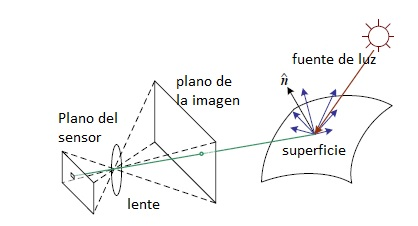
\includegraphics{Recursos/fotometria.jpg}
        \caption{Modelo simplificado fotométrico de la formación de imágenes}
        \label{photometry}
    \end{figure}
    \item \textbf{La resolución:} es un parámetro propio de la cámara que indica la cantidad de detalles que puede observarse en esta. En imágenes digitales la resolución es indicada mediante números enteros, donde el primero es la cantidad de columnas de píxeles (cuántos píxeles tiene la imagen a lo ancho) y el segundo es la cantidad de filas de píxeles (cuántos píxeles tiene la imagen a lo alto). Este factor tiene un nivel de relevancia variable dependiendo  campo de aplicación.
    \item Campo de visión o field of view (FOV): Es el ángulo abarcable por el sensor de una cámara para detectar la radiación electromagnética que se desee capturar. El campo de visión depende de la distancia focal de una cámara y esta dado por la siguiente ecuación:
    \begin{equation}
        \phi = tan^{-1}\left(\frac{d/2}{f}\right)
    \end{equation}
    En la Figura \ref{FOV} se pueden apreciar los elementos de interés para poder calcular el campo de visión de una cámara.
    \begin{figure}[H]
        \centering
        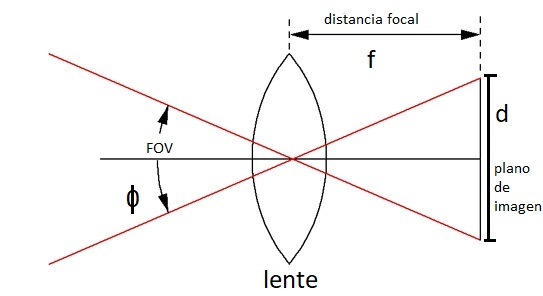
\includegraphics{Recursos/FOV.jpg}
        \caption{Campo de visión (FOV) de una cámara}
        \label{FOV}
    \end{figure}
    \item El posicionamiento relativo de las cámaras: se refiere a la ubicación en el espacio de una cámara respecto al resto del sistema de adquisición de datos. Depende de la complejidad del dominio de la escena o el campo de aplicación y afecta en el calculo del modelo de la cámara, el cual se detallara a profundidad en la siguiente sección.
    \item Oclusión: es un situación que ocurre con mayor frecuencia al emplearse dos o más cámaras, debido a la obstrucción parcial del objetivo, para una de las cámaras, mientras que el resto es capaz de observar al objetivo, pues este es un problema que el sistema de visión debe ser capaz de interpretar o canalizar para así realizar el paso 4 de visión estéreo de forma adecuada.
\end{itemize}
\subsection{Modelado de la Cámara}
\subsubsection{Sistema de coordenadas homogéneas y matriz homogenea}
Es una herramienta introducida por Forest en 1969 para resolver diferentes problemas de gráficos por computador a través de operaciones con matrices. Este tipo de transformaciones son empleadas para determinar en una sola matriz la posición y orientación de un objeto respecto a un sistema de referencia \cite{RSSFernando_homogeneusC}.

Cuando se emplean coordenadas homogéneas en imágenes, cada píxel tiene la siguiente representación:
\begin{equation}
(x, y) \Rightarrow
\begin{bmatrix}
x & y & 1
\end{bmatrix}^{T}
\end{equation}
Mientras que en el caso de una escena tridimensional la representación es:
\begin{equation}
(x, y, z) \Rightarrow
\begin{bmatrix}
x & y & z & 1
\end{bmatrix}^{T}
\end{equation}
Las traslaciones y rotaciones para las coordenadas homogéneas son operaciones lineales realizadas entre matrices, donde la nueva posición de un objeto, sera el producto entre la posición previa y la matriz de transformación. La matriz de transformación homogénea definida por Forest es de dimensiones 4x4 y esta compuesta a su vez por cuatro submatrices (Ecuación \ref{homogeneusMatrix}).
\begin{equation}
    T = \begin{bmatrix}
        \begin{array}{c|c}
                rotaci\acute{o}n & traslaci\acute{o}n\\
                \hline
                perspectiva & escalado
        \end{array}
        \end{bmatrix}
        =
        \begin{bmatrix}
        \begin{array}{c|c}
                3 x 3 & 3 x 1\\
                \hline
                1 x 3 & 1 x 1
        \end{array}
        \end{bmatrix}
\label{homogeneusMatrix}
\end{equation}
No obstante la matriz de transformación para 2D es de dimensiones 3 x 3 y tiene la siguiente representación:
\begin{equation}
    T = \begin{bmatrix}
        \begin{array}{c|c}
                rotaci\acute{o}n & traslaci\acute{o}n\\
                \hline
                perspectiva & escalado
        \end{array}
        \end{bmatrix}
        =
        \begin{bmatrix}
        \begin{array}{c|c}
                2 x 2 & 2 x 1\\
                \hline
                1 x 2 & 1 x 1
        \end{array}
        \end{bmatrix}
\end{equation}
Cuando se emplean coordenadas homogeneas no solo es más eficaz a nivel computacional, ya que permite efectuar cambios en la posición y orientación mediante productos matriciales, estas incluso se pueden convertir en coordenadas convencionales mediante una simple operación de división como en las siguientes expresiones:
\begin{align}
\begin{bmatrix}
x & y & w
\end{bmatrix}^{T} \Rightarrow (x/w, y/w)\label{homogeneus2d}\\
\begin{bmatrix}
x & y & z & w
\end{bmatrix}^{T} \Rightarrow (x/w, y/w, z/w)\label{homogeneus3d}
\end{align}
La ecuación \ref{homogeneus2d} se utiliza para convertir un píxel de una imagen 2D que se encuentra en coordenadas homogéneas a cartesianas, mientras que la ecuación \ref{homogeneus3d} se utiliza en el caso de tres dimensiones.
\subsection{Modelo de pinhole}
Es un modelo de cámara donde cada punto de un objeto situado en el entorno de trabajo (espacio tridimensional) se proyecta en un punto de un plano denominado plano imagen ó plano de proyección. En la Figura \ref{pinholeModel} ``PP'' es el plano de proyección y ``COP'' se refiere al centro de proyección o centro óptico de la cámara. El punto en la escena 3D se denota como $p^{M}$, dicho punto se encuentra en las coordenadas del mundo $p^{M}$ $(x, y, z)$ y su proyección en el plano de imagen se denota como $p^{I}$ $(x', y')$ y corresponde con la intersección entre la linea que une $p^{M}$ y COP con el plano de imagen, además a la distancia entre el plano de proyección y COP se le conoce como distancia focal. 
\begin{figure}[H]
    \centering
    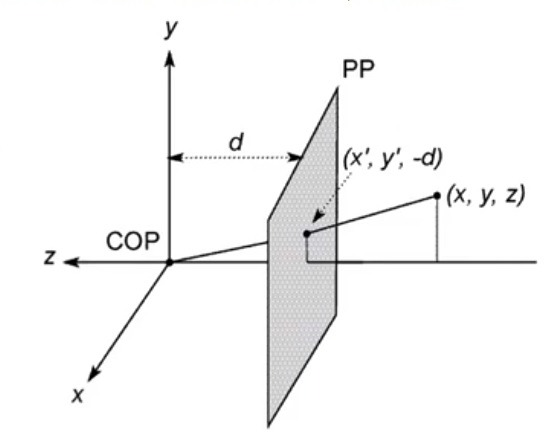
\includegraphics[scale=0.5]{Recursos/pinholeModel.jpg}
    \caption{Modelo de cámara pinhole}
    \label{pinholeModel}
\end{figure}
La razón del porque en el modelo presentado en la Figura \ref{pinholeModel} el plano de proyección se encuentra por delante del lente (a pesar de que en la realidad la luz ingresa a través del punto focal y luego impacta con el plano de imagen) es porque matemáticamente es más conveniente, debido a que de esta forma las imágenes no son invertidas.

Utilizando el teorema de Tales es posible determinar las proyecciones de los puntos en el plano de forma tal que se cumple la siguiente ecuación:
\begin{equation}
    (X, Y, Z) \longrightarrow (-d\frac{X}{Z}, -d\frac{Y}{Z}, -d)  \label{convert3Dto2Dpinhole}
\end{equation}
La operación realizada en la ecuación \ref{convert3Dto2Dpinhole}, permite proyectar los puntos del espacio 3D en el plano de imagen, dicha operación puede ser realizada mediante coordenadas homogéneas de la siguiente forma:
\begin{align}
            \begin{bmatrix}
            1 & 0 & 0 & 0\\
            0 & 1 & 0 & 0\\
            0 & 0 & 1/f & 0
            \end{bmatrix}
            \begin{bmatrix}
            x\\
            y\\
            z\\
            1
            \end{bmatrix}
            =
            \begin{bmatrix}
            x\\
            y\\
            z/f\\
            \end{bmatrix} \Rightarrow \left(-f\frac{X}{Z}, -f\frac{Y}{Z}\right)\label{convert3Dto2Dperspective}
\end{align}
A la forma en la que se proyecta en la ecuación \ref{convert3Dto2Dperspective} se le conoce como proyección de perspectiva y esta llega al mismo resultado que el de la ecuación \ref{convert3Dto2Dpinhole}, ya que $f$ es la distancia focal.
\subsection{Parámetros intrínsecos y extrínsecos}
\subsubsection{Parámetros intrínsecos}
\subsubsection{Parámetros extrínsecos}
